% !TeX program = lualatex
% !TeX encoding = utf8
% !TeX spellcheck = uk_UA

\documentclass[10pt]{beamer}
\usetheme{QuantumChemistry}
\usepackage{QuantumChemistry}
%\usepackage{unicode-math-luatex}
%\usepackage{makecell, booktabs, pgf}
%\usepackage{minted, xcolor}
\graphicspath{{pictures/}}
\addbibresource{bibliography.bib}


\title[Лекції з квантової хімії]{{\bfseries\huge Два електрони в одновимірній потенціальній ямі} \\ {Прообраз багатоелектронної системи}}
\author{Пономаренко С. М.}
\subtitle{Лекції з квантової хімії}
\date{}
\begin{document}
%%==============================================================================
%\usebackgroundtemplate{
%	\tikz\node[opacity=0.1]{\includegraphics[width=\paperwidth,height=\paperheight]{background}};%
%}


\begin{frame}
	\thispagestyle{empty}
	\titlepage
\end{frame}

%============================================================================
\begin{frame}{Що треба вияснити при розв'язку задачі?}{}
    \begin{block}{}
    	\begin{enumerate}
    		\item Як розв'язати рівняння Шредінґера?
    		      \begin{itemize}
    			      \item Як спростити?
    			      \item Як розділити змінні?
    		      \end{itemize}
    		\item Як виглядає хвильова функція системи?
    		\item Який сенс вона має?
    		\item Як розподілений заряд в системі (для молекул це особливо цікаво)?
    	\end{enumerate}
    \end{block}
	\begin{center}
		\includegraphics[width=3cm]{Charge_in_water_molecule}
	\end{center}
\end{frame}
%============================================================================

%============================================================================
\begin{frame}{Рівняння Шредінґера}{}
	\begin{equation*}
		\tcbhighmath{\hat{H}\Phi(x_1, x_2) = E\Phi(x_1, x_2).}
	\end{equation*}
	\begin{columns}
		\begin{column}{0.3\linewidth}\centering
			\begin{tikzpicture}[scale=0.95]
				\def\l{3}
				\def\h{4}
				\draw[->] (0,-0.5) -- (0,{\h + 0.5}) node[left] {$U$};
				\draw[->] (-0.5,0) -- ({\l + 0.5},0) node[below] {$x$};
				\fill[pattern=north east lines] (-0.125, 0) rectangle (0, \h);
				\draw[] (\l,-0.5) -- (\l,{\h + 0.5});
				\fill[pattern=north west lines] (\l, 0) rectangle ({\l + 0.125}, \h);
				\draw[<->] (0,-0.3) -- node[below] {$l$} ++(\l,0);
				\draw[ball color = red] ({\l/4}, {1^2}) circle (0.05);
				\draw[ball color = red] ({3*\l/4}, {1^2}) circle (0.05);
			\end{tikzpicture}
		\end{column}
		\begin{column}{0.7\linewidth}\centering
			\begin{block}{}
                Гамільтоніан системи:
       			\begin{equation*}
       				\hat{H} = -\frac12 \frac{\partial^2}{\partial x_1^2}  - \frac12 \frac{\partial^2}{\partial x_2^2}  + \frac{1}{|x_1 - x_2|}.
       			\end{equation*}
       			Спрощення --- нехтуємо взаємодією електронів
               \begin{equation*}
                    \frac{1}{|x_1 - x_2|} = 0.
               \end{equation*}
       			Незалежність руху електронів --- розділяємо змінні
                \begin{equation*}
                    \Phi(x_1, x_2) = \phi_{n_1}(x_1) \phi_{n_2}(x_2).
                \end{equation*}
            \end{block}
		\end{column}
	\end{columns}
\end{frame}

%============================================================================
\begin{frame}{Стани електронів в потенціальній ямі}{Невзаємодіючі електрони}
	\begin{equation*}
		\phi_{n_1}(x_1) = \sqrt{\frac{2}{l}} \sin \left( n_1 \frac{\pi x_1}{l} \right) , \,
		\phi_{n_2}(x_2) = \sqrt{\frac{2}{l}} \sin \left( n_2 \frac{\pi x_2}{l} \right) , \,
		E = \frac{\pi^2}{2l^2}(n_1^2 + n_2^2)
	\end{equation*}
	\begin{columns}
		\begin{column}{0.5\linewidth}\centering
			\begin{tikzpicture}[scale=0.95]
				\def\l{3}
				\def\h{4}
				\draw[->] (0,-0.5) -- (0,{\h + 0.5}) node[left] {$U$};
				\draw[->] (-0.5,0) -- ({\l + 0.5},0) node[below] {$x$};
				\fill[pattern=north east lines] (-0.125, 0) rectangle (0, \h);
				\draw[] (\l,-0.5) -- (\l,{\h + 0.5});
				\fill[pattern=north west lines] (\l, 0) rectangle ({\l + 0.125}, \h);
				\draw[<->] (0,-0.3) -- node[below] {$l$} ++(\l,0);
				\foreach \i[count = \c from 1] in {0.5, 1, ..., 2}
					{
						\draw[red] (0, {\i^2}) -- ++(\l, 0) node[left=5pt, pos=0, font=\small, color=gray] {$n = \c$};
						\draw[variable=\x, domain=0:\l, samples=50, gray] plot (\x, {\i^2 + 0.25*sin(deg(\c*pi*\x/\l))});
						%\draw[ball color = red] ({\l/4}, {\i^2}) circle (0.05);
						%\draw[ball color = red] ({3*\l/4}, {\i^2}) circle (0.05);
					}
			\end{tikzpicture}
		\end{column}
		\begin{column}{0.5\linewidth}\centering
			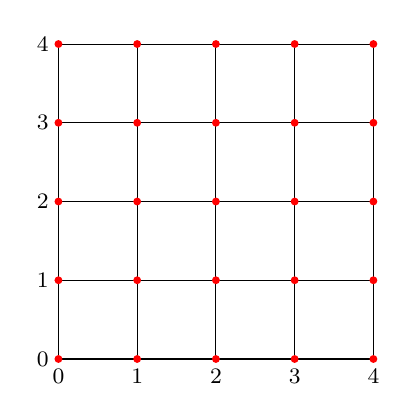
\begin{tikzpicture}
				\def\w{4}
				\draw[step=1.0,black,thin] (0,0) grid (\w,\w);
				\foreach \i in {0,...,\w}
					{
						\node[left, font = \footnotesize] at (0, \i) {$\i$};
						\node[below, font = \footnotesize] at (\i, 0) {$\i$};
						\foreach \j in {0,...,\w}
							{
								\fill[red] (\i, \j) circle (0.05);
							}
					}
			\end{tikzpicture}
		\end{column}
	\end{columns}
	\begin{alertblock}{}\centering
		Функція системи двох електронів \(\Phi(x_1, x_2) = \phi_{n_1}(x_1) \phi_{n_2}(x_2)\) ?
	\end{alertblock}
\end{frame}
%============================================================================

% ============================== Слайд ## ===================================
\begin{frame}{Симетричні та антисиметричні функції}{Тотожність частинок}
	\begin{onlyenv}<1>\small
		\begin{block}{Тотожність частинок}
			У мікросвіті частинки одного <<сорту>> тотожні не тільки в тому сенсі, що їхні властивості (маса спокою, заряд \ldots) точно збігаються між собою, а в тому сенсі, що \alert{перестановка місцями двох довільних частинок в системі не призводить до зміни фізичного стану системи}.
		\end{block}
		\begin{alertblock}{}
			Власні значення операторів фізичних величин не повинні залежати від нумерації частинок!
		\end{alertblock}
		\begin{block}{}
			Хвильова функція має задовольняти одному й тому самому рівнянню Шредінгера при зміні частинок місцями (при цьому не змінюється також і власне
			значення енергії):
			\begin{align*}
				\hat{H}\Phi(x_1, x_2) & = E\Phi(x_1, x_2), \\
				\hat{H}\Phi(x_2, x_1) & = E\Phi(x_2, x_1).
			\end{align*}
		\end{block}
	\end{onlyenv}
	\begin{onlyenv}<2>
		\begin{block}{}\justifying
			При перестановці частинок функція системи може змінитись лише на фазовий множник $e^{i\alpha}$ (це не змінює стану системи згідно квантової механіки)
			\begin{equation*}
				\Phi(x_1, x_2) = e^{i\alpha}\Phi(x_2, x_1)
			\end{equation*}
			Повторна перестановка дає:
			\begin{equation*}
				\Phi(x_1, x_2) = e^{2i\alpha}\Phi(x_1, x_2).
			\end{equation*}
			Звідки
			\begin{equation*}
				e^{2i\alpha} = 1, \quad e^{i\alpha} = \pm 1.
			\end{equation*}
			Тобто хвильова функція при перестановці може змінити лише знак.
		\end{block}
		\begin{block}{}
			Функції які змінюють знак при перестановці --- \alert{антисиметричні}, які не змінюють --- \alert{симетричні}.
		\end{block}
	\end{onlyenv}
	\begin{onlyenv}<3>
		\begin{block}{}
			Оператор перестановки частинок:
			\begin{equation*}
				\hat{P}\Phi(x_1, x_2) = \lambda\Phi(x_2, x_1).
			\end{equation*}
			Повторна перестановка дає:
			\begin{equation*}
				\hat{P}^2\Phi(x_1, x_2) = \lambda^2\Phi(x_1, x_2), \quad \lambda =  \pm 1.
			\end{equation*}

			Власні значення оператора перестановки не може залежати від перестановки частинок, отже хвильова функція системи тотожних частинок має бути симетричною або антисиметричною щодо операції перестановки цих частинок.
		\end{block}
	\end{onlyenv}
\end{frame}
% ===========================================================================


\begin{frame}{Спін електрона}{Досліди Штерна-Герлаха}
	\begin{center}
		\alert{Спін електрона --- внутрішній момент імпульсу.}
	\end{center}
	\begin{columns}
		\begin{column}{0.5\linewidth}\centering
			Базисні спінові стани електрона
			\[\gamma = \{\alpha \text{ або } \uparrow, \beta \text{ або } \downarrow\}\]
			Квадрат модуля вектора спіну
			\begin{equation*}\label{}
				\tcbhighmath{\hat{s}^2 \gamma = s (s + 1) \gamma.}
			\end{equation*}
			Число проекцій на вісь $z$
			\[
				2 = 2 s + 1 \quad  \Rightarrow \quad s = \frac{1}{2}.
			\]
			\begin{equation*}\label{}
				\hat{s}_{z} \alpha = +\frac12 \alpha, \quad   \hat{s}_{z} \beta = -\frac12 \beta.
			\end{equation*}
		\end{column}
		\begin{column}{0.5\linewidth}\centering
			\includegraphics[width=1\linewidth]{SternHerlach}\\
			\includegraphics[width=0.75\linewidth]{Spin}
		\end{column}
	\end{columns}
\end{frame}
%============================================================================
\begin{frame}{Оператор спіну}{Матриці Паулі --- наслідок експериментів Штерна-Герлаха}\centering
	\begin{columns}
		\begin{column}{0.5\linewidth}\centering
			Оператори проекцій спіну:
			\begin{equation*}\label{}
				\hat{s}_{z} \alpha = +\frac12 \alpha, \quad   \hat{s}_{z} \beta = -\frac12 \beta.
			\end{equation*}
			Матриці Паулі:
			\begin{align*}\label{}
				\hat{\sigma}_{z} \alpha =  \alpha, \quad  & \hat{\sigma}_{z} \beta = \beta,    \\
				\hat{\sigma}_{x} \alpha =  \beta, \quad   & \hat{\sigma}_{x} \beta = \alpha,   \\
				\hat{\sigma}_{y} \alpha =  i \beta, \quad & \hat{\sigma}_{y} \beta = -i\alpha.
			\end{align*}
			Оператор вектора спіну:
			\begin{multline*}\label{}
				\hat{\vec{s}}  =  \hat{s}_{x} \vec{e}_x + \hat{s}_{y} \vec{e}_y + \hat{s}_{z} \vec{e}_z = \\ = \frac12 \left( \hat{\sigma}_{x} \vec{e}_x + \hat{\sigma}_{y} \vec{e}_y + \hat{\sigma}_{z} \vec{e}_z \right)  = \frac12\vec{\sigma}
			\end{multline*}
		\end{column}
		\begin{column}{0.5\linewidth}\centering
			\includegraphics[width=0.75\linewidth]{PauliWrite}

			\href{https://www.youtube.com/watch?v=ou9JNBZJDiM}{\button{Матриці Паулі}}

            \bigskip

			Рівняння Паулі:
			\begin{equation*}
            \tcbhighmath{%
				\left[\hat{H}_0  - \frac{e}{mc} \left(\frac\hbar2\hat{\vec{\sigma}} \cdot \vec{B}\right)\right] \Psi = i\hbar \frac{\partial \Psi}{ \partial t} .
                }
			\end{equation*}
		\end{column}
	\end{columns}
\end{frame}
%============================================================================

\begin{frame}{Спін системи двох електронів}{\alert{Кількість проекцій на вісь $z$ ---  мультиплетність.}}\centering
	Вектор спіну системи двох електронів:
	\(
	\hat{\vec{s}} = \hat{\vec{s}}_1 + \hat{\vec{s}}_2.
	\)

	\medskip

	Проекція спіну системи двох електронів на вісь $z$:
	\(
	\hat{s}_z = \hat{s}_{z_1} + \hat{s}_{z_2}.
	\)
	\begin{overprint}

		\bigskip

		\onslide<1>
		\begin{center}
			\alert{Антисиметрична спінова функція двох електронів}
		\end{center}
		\onslide<2>
		\begin{center}
			\alert{Симетричні спінові функції двох електронів}
		\end{center}
	\end{overprint}

	\medskip

	\begin{columns}\small
		\begin{column}{0.7\linewidth}
			\begin{overprint}\centering
				\onslide<1>
				\begin{equation*}
					\gamma^{A} = \frac1{\sqrt2} \left[ \alpha(1) \beta(2) - \alpha(2) \beta(1) \right]
				\end{equation*}
				\begin{align*}
					\hat{\vec{s}}\, \gamma^{A} & = 0\, \gamma^{A}, \\
					\hat{s}^2 \gamma^{A}       & = 0\, \gamma^{A}, \\
					\quad \hat{s}_z \gamma^{A} & = 0\, \gamma^{A}.
				\end{align*}
				\onslide<2>
				\begin{align*}
					\gamma^{S}_1 & = \alpha(1) \alpha(2),                                                    \\
					\gamma^{S}_2 & = \frac1{\sqrt2} \left[ \alpha(1) \beta(2) + \alpha(2) \beta(1) \right] , \\
					\gamma^{S}_3 & = \beta(1) \beta(2).
				\end{align*}
				\begin{equation*}
					\hat{s}^2 \gamma^{S}_{1,2,3} = 1\cdot (1 + 1)\, \gamma^{S}_{1,2,3}.
				\end{equation*}
				\begin{align*}
					\hat{s}_z \gamma^{S}_1 & = +1\, \gamma^{S}_2, \\
					\hat{s}_z \gamma^{S}_2 & = 0\,  \gamma^{S}_2, \\
					\hat{s}_z \gamma^{S}_3 & = -1\, \gamma^{S}_3
				\end{align*}
			\end{overprint}
		\end{column}
		\begin{column}[c]{0.3\linewidth}\centering
			\begin{overprint}
				\onslide<1>
				\includegraphics[width=0.75\linewidth]{SpinAdd1}
				\onslide<2>
				\includegraphics[width=0.75\linewidth]{SpinAdd2}
			\end{overprint}
		\end{column}
	\end{columns}

	\bigskip

	\begin{overprint}
		\onslide<1>
		\begin{center}
			\alert{Мультиплетність $M = 2s + 1 = 1$ \(\Rightarrow\) синглет}
		\end{center}
		\onslide<2>
		\begin{center}
			\alert{Мультиплетність $M = 2s + 1 = 3$ \(\Rightarrow\) триплет}
		\end{center}
	\end{overprint}
\end{frame}

%============================================================================

\begin{frame}{Принцип Паулі}{сформульовано Вольфгангом Паулі 1925 року }
	\begin{columns}
		\begin{column}{0.3\linewidth}
			\begin{center}
				\includegraphics[width=1\linewidth]{Pauli}
			\end{center}
		\end{column}
		\begin{column}{0.7\linewidth}
			%			\begin{block}{Принцип тотожності частинок}\small
			%				В просторі де хвильові функції двох і більше частинок перекриваються --- то розрізнити, яка з них знаходиться в даній області, взагалі немає сенсу: можна говорити лише про ймовірність знаходження в даній області однієї з тотожних частинок.
			%			\end{block}
			\begin{block}{Принцип Паулі}\small
				Хвильова функція електронів має бути \alert{антисиметричною} по відношенню до перестановки місцями двох  довільних частинок:
				\begin{equation*}
					\Phi (\vxi_1, \vxi_2) = - \Phi (\vxi_2, \vxi_1)
				\end{equation*}
			\end{block}
		\end{column}
	\end{columns}
\end{frame}

%============================================================================

\begin{frame}{Врахування антисиметрії хвильової функції}
	Хвильова функція двох невзаємодіючих електронів:
	\begin{equation*}
		\Phi(\vxi_1, \vxi_2) ={1}/{\sqrt2}\left[\vphi_{n_1}(\vxi_1)\vphi_{n_2}(\vxi_2) -\vphi_{n_1}(\vxi_2)\vphi_{n_2}(\vxi_1)\right]
	\end{equation*}
	\begin{overprint}
		\framesubtitle<1>{Детермінант Слейтера і принцип заборони Паулі}
		\onslide<1>%
		\begin{block}{Детермінант Слейтера}
			Таку антисиметричну двоелектронну функцію можна також представити у вигляді детермінанта:
			\begin{equation*}
				\Phi (\vxi_1, \vxi_2)={\frac {1}{\sqrt {2}}}
				\left|
				{
				\begin{matrix}
					\vphi_{n_1}(\vxi_1) & \vphi_{n_2}(\vxi_1) \\
					\vphi_{n_1}(\vxi_2) & \vphi_{n_2}(\vxi_2)
				\end{matrix}
				}
				\right|.
			\end{equation*}
			Якщо два електрона займають однаковий стан ($n_1 = n_2$) $\rightarrow$ детермінант дорівнює $0$.
		\end{block}
		\begin{block}{Принцип заборони Паулі}
			Жодна пара електронів  не може займати однаковий стан.
		\end{block}
		\framesubtitle<2>{Спін-орбіталі та орбіталі}
		\onslide<2>%
		Одноелектронна функція називається \alert{спін-орбіталлю}, оскільки вона залежить як від спінових змінних $\sigma$  так і від просторових координат~$\vec{r}$.

		\begin{equation*}\label{spin-orbit}
			\vphi_{n_i}(\vxi_i) = \vphi_{n_i}(\vr_i, \sigma_i),
		\end{equation*}

		Так як гамільтоніан не враховує спін-орбітальну взаємодію, то спін-орбіталь в свою чергу можна представити у вигляді добутку координатної та спінової функцій:
		\begin{equation*}
			\vphi_{n_i}(\vec{r}_i, \sigma_i) = \phi_{n_i}(\vec{r}_i) \gamma_{n_i}(\sigma_i), \quad \text{де } \gamma = \alpha (\text{ або }\uparrow), \beta (\text{ або }\downarrow)
		\end{equation*}
		Координатна функція $\phi_{n_i}(\vec{r}_i)$ називається \alert{орбіталлю}.
		\framesubtitle<3>{Як отримати хвильову функцію системи?}
		\onslide<3>\small
		Для отримання хвильової функції необхідно:
		\begin{enumerate}
			\item  Розв'язати рівняння Шредінґера:
			      \begin{equation*}
				      \hat{H}\Phi(\vxi_1, \vxi_2) = E\Phi(\vxi_1, \vxi_2).
			      \end{equation*}
			\item Для невзаємодіючих частинок рівняння розпадається на два (по числу електронів):
			      \begin{align*}
				      \hat{h}_1\vphi_{n_1}(\vxi_1) & = \varepsilon_1\vphi_{n_1}(\vxi_1), \\
				      \hat{h}_2\vphi_{n_2}(\vxi_2) & = \varepsilon_2\vphi_{n_2}(\vxi_2).
			      \end{align*}
			\item Стаціонарні розв'язки рівняння Шредінґера системи формують із знайдених спін-орбіталей $\{\vphi_{n_1}(\vxi_1)\}$ та $\{\vphi_{n_2}(\vxi_2)\}$ у вигляді детермінантів $2\times2$ (або їх суперпозиції), кожен з яких буде власною функцією оператора $\hat{H}$.
		\end{enumerate}
	\end{overprint}
\end{frame}
%============================================================================2





%============================================================================
\begin{frame}{Приклади побудови детермінантів Слейтера}
	\begin{center}
		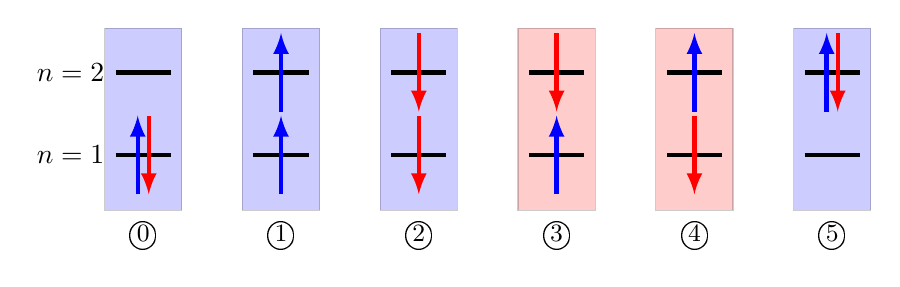
\begin{tikzpicture}[scale=0.7,
				upspinarrow/.pic = {\draw[-latex, blue] (0,-0.5) -- (0, 0.5);},
				downspinarrow/.pic = {\draw[latex-,red] (0,-0.5) -- (0, 0.5);}
			]
			\def\yshiftnode{-1.5}
			\def\xshiftnode{0.5}
			\def\distance{1.5}
			\draw<1> [fill=blue, opacity=0.2] (-0.20,-1) rectangle (1.20,2.3);
			%			\draw<7-> [fill=red, opacity=0.2] (-0.20,-1) rectangle (1.20,2.3);
			\draw[ultra thick]  (0,0) node[left] {$n = 1$} -- pic[pos=0.4] {upspinarrow}  pic[pos=0.6] {downspinarrow}+(1,0);
			\draw[ultra thick]  (0,\distance) node[left] {$n = 2$} -- +(1,0);
			\node at (\xshiftnode,\yshiftnode) {\textcircled{\small{0}}};
			\begin{scope}[xshift=2.5cm]
				\draw<2> [fill=blue, opacity=0.2] (-0.20,-1) rectangle (1.20,2.3);
				\draw[ultra thick]  (0,0) -- pic {upspinarrow}  +(1,0);
				\draw[ultra thick]  (0,\distance) -- pic {upspinarrow} +(1,0);
				\node at (\xshiftnode,\yshiftnode) {\textcircled{\small{1}}};
			\end{scope}
			\begin{scope}[xshift=5cm]
				\draw<3> [fill=blue, opacity=0.2] (-0.20,-1) rectangle (1.20,2.3);
				\draw[ultra thick]  (0,0) -- pic {downspinarrow}  +(1,0);
				\draw[ultra thick]  (0,\distance) -- pic {downspinarrow} +(1,0);
				\node at (\xshiftnode,\yshiftnode) {\textcircled{\small{2}}};
			\end{scope}
			\begin{scope}[xshift=7.5cm]
				\draw<4-5> [fill=red, opacity=0.2] (-0.20,-1) rectangle (1.20,2.3);
				\draw[ultra thick]  (0,0) -- pic {upspinarrow}  +(1,0);
				\draw[ultra thick]  (0,\distance) -- pic {downspinarrow} +(1,0);
				\node at (\xshiftnode,\yshiftnode) {\textcircled{\small{3}}};
			\end{scope}
			\begin{scope}[xshift=10cm]
				\draw<4-5> [fill=red, opacity=0.2] (-0.20,-1) rectangle (1.20,2.3);
				\draw[ultra thick]  (0,0) -- pic {downspinarrow}  +(1,0);
				\draw[ultra thick]  (0,\distance) -- pic {upspinarrow} +(1,0);
				\node at (\xshiftnode,\yshiftnode) {\textcircled{\small{4}}};
			\end{scope}
			\begin{scope}[xshift=12.5cm]
				\draw<6> [fill=blue, opacity=0.2] (-0.20,-1) rectangle (1.20,2.3);
				\draw[ultra thick]  (0,0) -- +(1,0);
				\draw[ultra thick]  (0,\distance) -- pic[pos=0.4] {upspinarrow}  pic[pos=0.6] {downspinarrow} +(1,0);
				\node at (\xshiftnode,\yshiftnode) {\textcircled{\small{5}}};
			\end{scope}
		\end{tikzpicture}
	\end{center}
	\begin{overprint}
		\onslide<1>
		Для випадку {\textcircled{\small{0}}\/}:
		\begin{equation*}
			\Phi_0 ={\frac {1}{\sqrt {2}}}
			\left|
			{
			\begin{matrix}
				\phi_1(1)\alpha(1) & \phi_1(2)\alpha(2) \\
				\phi_1(1)\beta(1)  & \phi_1(2)\beta(2)
			\end{matrix}
			}
			\right| = {\frac {1}{\sqrt {2}}} \phi_1(1) \phi_1(2) \left[\alpha(1)\beta(2) - \alpha(2)\beta(1)\right].
		\end{equation*}
		Детермінант --- добуток симетричної координатної частини $\phi_S$ та антисиметричної спінової частини $\gamma_A^0 $. Верхній індекс <<$0$>> --- повний спін системи дорівнює нулю.
		\begin{equation*}\label{ground_state_parahelium_spin}
			\Phi_0 = \Phi_S \gamma_A^0.
		\end{equation*}
		\onslide<2>
		Для випадку {\textcircled{\small{1}}}:
		\begin{equation*}
			\Phi_1 ={\frac {1}{\sqrt {2}}}
			\left|
			{
			\begin{matrix}
				\phi_1(1)\alpha(1) & \phi_1(2)\alpha(2) \\
				\phi_2(1)\alpha(1) & \phi_2(2)\alpha(2)
			\end{matrix}
			}
			\right| = {\frac {1}{\sqrt {2}}} \alpha(1) \alpha(2) \left[\phi_1(1)\phi_2(2) -\phi_2(1)\phi_1(2)\right],
		\end{equation*}
		\begin{equation*}
			\Phi_1 = \Phi_A \gamma_S^{+1},
		\end{equation*}
		верхній індекс <<$+1$>> показує, що повний спін системи в цьому стані дорівнює $+1$.
		\onslide<3>
		Для випадку {\textcircled{\small{2}}}:
		\begin{equation*}
			\Phi_2 = {\frac {1}{\sqrt {2}}}
			\left|
			{
			\begin{matrix}
				\phi_1(1)\beta(1) & \phi_1(2)\beta(2) \\
				\phi_2(1)\beta(1) & \phi_2(2)\beta(2)
			\end{matrix}
			}
			\right| = {\frac {1}{\sqrt {2}}} \beta(1) \beta(2) \left[\phi_1(1) \phi_2(2) -\phi_2(1)\phi_1(2)\right]
		\end{equation*}
		\begin{equation*}
			\Phi_2= \Phi_A \gamma_S^{-1}
		\end{equation*}
		\onslide<4>
		Для випадків {\textcircled{\small{3}}} та {\textcircled{\small{4}}} не можна побудувати однодетермінантні функції, треба брати лінійні комбінації детермінантів.
		\onslide<5>
		Випадок {\textcircled{\small{3}}}
		$
			\Phi_3 = {\frac {1}{\sqrt {2}}} = (\Phi_I + \Phi_{II}) = \Phi_A \gamma_S^0,
		$

		Випадок {\textcircled{\small{4}}}:
		$
			\Phi_4 = {\frac {1}{\sqrt {2}}} = (\Phi_I - \Phi_{II}) = \Phi_S \gamma_A ^0 ,
		$

		\begin{equation*}
			\Phi_I = {\frac {1}{\sqrt {2}}}
			\left|
			{
			\begin{matrix}
				\phi_1(1)\alpha(1) & \phi_1(2)\alpha(2) \\
				\phi_2(1) \beta(1) & \phi_2(2)\beta(2)
			\end{matrix}
			}
			\right|, \quad
			\Phi_{II} = {\frac {1}{\sqrt {2}}}
			\left|
			{
			\begin{matrix}
				\phi_1(1) \beta(1) & \phi_1(2)\beta(2)  \\
				\phi_2(1)\alpha(1) & \phi_2(2)\alpha(2)
			\end{matrix}
			}
			\right|.
		\end{equation*}
		\onslide<6>
		Для випадку {\textcircled{\small{5}}}:
		\begin{equation*}
			\Phi_5 ={\frac {1}{\sqrt {2}}}
			\left|
			{
			\begin{matrix}
				\phi_2(1)\alpha(1) & \phi_2(2)\alpha(2) \\
				\phi_2(1) \beta(1) & \phi_2(2)\beta(2)
			\end{matrix}
			}
			\right| = {\frac {1}{\sqrt {2}}} \phi_2(1) \phi_2(2) \left[\alpha(1)\beta(2) - \beta(1)\alpha(2)\right].
		\end{equation*}
	\end{overprint}
\end{frame}
%============================================================================





%============================================================================
\begin{frame}{Основний стан двоелектронної системи}
	\framesubtitle<1>{Синглетний стан}
	\framesubtitle<2>{Триплетний стан}
	Хвильова функція двох невзаємодіючих електронів:
	\begin{equation*}
		\Phi(\vxi_1, \vxi_2) ={1}/{\sqrt2}\left[\vphi_{n_1}(\vxi_1)\vphi_{n_2}(\vxi_2) -\vphi_{n_1}(\vxi_2)\vphi_{n_2}(\vxi_1)\right]
	\end{equation*}
	\begin{overprint}
		\onslide<1>%
		Детермінант \alert{синглетного основного стану} невзаємодіючих електронів в станах $n_1 = n_2 = 1$ (\alert{однакова орбіталь}):

		\begin{multline*}
			\Phi (\vxi_1, \vxi_2)={\frac {1}{\sqrt {2}}}
			\left|
			{
			\begin{matrix}
				\phi_{1}(x_1) \alpha(1) & \phi_{1}(x_1) \beta(1) \\
				\phi_{1}(x_2) \alpha(2) & \phi_{1}(x_2) \beta(2)
			\end{matrix}
			}
			\right| = \\
			= 1/\sqrt2 \phi_1(x_1) \phi_1(x_2) \left[ \alpha(1) \beta(2) - \alpha(2)\beta(1)\right].
		\end{multline*}
		\begin{center}
			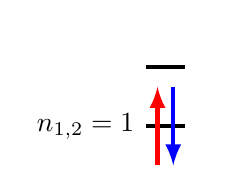
\begin{tikzpicture}[scale=0.5, baseline = (base),
					upspinarrow/.pic = {\draw[-latex, red] (0,-0.5) -- (0, 0.5);},
					downspinarrow/.pic = {\draw[latex-,blue] (0,-0.5) -- (0, 0.5);}
				]
				\def\distance{1.5}
				\draw[ultra thick]  (0,0) node[left] {$n_{1,2} = 1$} -- pic[pos=0.3] {upspinarrow}  pic[pos=0.7] {downspinarrow}+(1,0);
				\draw[ultra thick]  (0,\distance) -- +(1,0);
				\path (-1.5, -1) rectangle (1.5,2.5);
				\coordinate (base) at (-1.5, 0);
			\end{tikzpicture}
		\end{center}
		\onslide<2>%
		Детермінант \alert{триплетного основного стану} невзаємодіючих електронів з проекціями спінів $\uparrow\uparrow$ в станах $n_1 = 1$, $n_2 = 2$ (\alert{різні орбіталі}).

		%        Випадок  $\uparrow\uparrow$:
		\begin{multline*}
			\Phi (\vxi_1, \vxi_2)={\frac {1}{\sqrt {2}}}
			\left|
			{
			\begin{matrix}
				\phi_{1}(x_1) \alpha(1) & \phi_{2}(x_1) \alpha(1) \\
				\phi_{1}(x_2) \alpha(2) & \phi_{2}(x_2) \alpha(2)
			\end{matrix}
			}
			\right| = \\
			= 1/\sqrt2 \left[ \phi_1(x_1) \phi_2(x_2) -  \phi_1(x_2) \phi_2(x_1) \right] \alpha(1) \alpha(2).
		\end{multline*}
		\begin{center}
			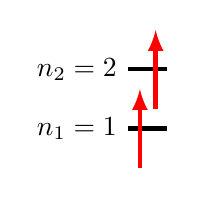
\begin{tikzpicture}[scale=0.5, baseline = (base),
					upspinarrow/.pic = {\draw[-latex, red] (0,-0.5) -- (0, 0.5);},
					downspinarrow/.pic = {\draw[latex-,blue] (0,-0.5) -- (0, 0.5);}
				]
				\def\distance{1.5}
				\draw[ultra thick]  (0,0) node[left] {$n_1 = 1$} -- pic[pos=0.3] {upspinarrow}  +(1, 0);
				\draw[ultra thick]  (0,\distance) node[left] {$n_2 = 2$} -- pic[pos=0.7] {upspinarrow} +(1,0);
				\path (-1.5, -1) rectangle (1.5,2.5);
				\coordinate (base) at (-1.5, 0);
			\end{tikzpicture}
		\end{center}

		%        Випадок  $\downarrow\downarrow$:
		%		\begin{equation*}
		%			\Phi (\vxi_1, \vxi_2)={\frac {1}{\sqrt {2}}} = \sqrt2 \left[ \phi_1(x_1) \phi_2(x_2) -  \phi_1(x_2) \phi_2(x_1) \right] \beta(1) \beta(2).
		%		\end{equation*}
		%
		%        Випадок  $\uparrow\downarrow$:
		%		\begin{equation*}
		%			\Phi (\vxi_1, \vxi_2)={\frac {1}{\sqrt {2}}} = \sqrt2 \left[ \phi_1(x_1) \phi_2(x_2) -  \phi_1(x_2) \phi_2(x_1) \right] \left[ \alpha(1) \beta(2) + \alpha(2)\beta(1)\right].
		%		\end{equation*}
	\end{overprint}
\end{frame}

%============================================================================

%============================================================================
\begin{frame}{Розподіл електронної густини}{}
	Заряд системи двох електронів $N_e = 2$:
	\begin{equation*}
		\int\limits_{V} \rho(x,y,z) dxdyxz = N_e \,\text{(сумарний заряд)}
	\end{equation*}
	Квадрат модуля хвильової функції:
	\begin{equation*}
		\int\limits_{V_1} \int\limits_{V_2} \int\limits_{\sigma_1} \int\limits_{\sigma_2} |\Phi (\vxi_1, \vxi_2)|^2  dV_1 dV_2 d\sigma_1d\sigma_2 = 1
	\end{equation*}
	Квадрат модуля орбіталей $\int |\phi(x,y,z)|^2 dV = 1$.\\
	Квадрат модуля спінових станів $\int |\alpha|^2 d\sigma = \int |\beta|^2 d\sigma = 1$, $\int \beta \alpha d\sigma = 0$.\\
	Розподіл електронної густини:
	\begin{equation*}
		\rho(x,y,z) = N_e  \int\limits_{V_2} \int\limits_{\sigma_1} \int\limits_{\sigma_2} |\Phi (\vxi_1, \vxi_2)|^2  dV_2 d\sigma_1d\sigma_2 = |\phi_1(x,y,z)|^2 + |\phi_2(x,y,z)|^2.
	\end{equation*}
\end{frame}

%============================================================================
\begin{frame}{Задачі}{}
%	\begin{enumerate}
%		\item Записати явний вигляд функції системи двох електронів в одновимірній потенціальній ямі для основного синглетного та триплетного стану (три функції).
%		\item Знайти розподіл електронної густини системи двох електронів в одновимірній потенціальній ямі для основного синглетного та триплетного стану.
%	\end{enumerate}
    \begin{enumerate}
    \item Запишіть детермінант Слейтера для основного стану системи трьох частинок (прикладом може бути основний стан атома \ce{Li}). Яка мультиплетність основного стану?
    \item Знайдіть вираз електронної густини для цього випадку через орбіталі використовуючи формулу:
    	\begin{equation*}
    		\rho(x,y,z) = 3  \int\limits_{V_2}  \int\limits_{V_3} \int\limits_{\sigma_1} \int\limits_{\sigma_2} \int\limits_{\sigma_3}  |\Phi (\vxi_1, \vxi_2, \vxi_3)|^2  dV_2dV_3 d\sigma_1d\sigma_2d\sigma_3.
    	\end{equation*}
    \item Зробіть висновки з попереднього розв'язку: як має виглядати електронна густина для системи $N_e$ електронів (виведення для загальному випадку робити не треба)?
    \end{enumerate}
\end{frame}
%============================================================================


\begin{frame}{}{}\centering
	\frametitle<1,3>{Синглетний стан}
	\frametitle<2>{Триплетний стан}
	\framesubtitle<1-2>{Невзаємодіючі електрони}
	\framesubtitle<3>{Взаємодіючі електрони}
	\only<1>{%
		\begin{equation*}
			\Phi_0(\xi_1, \xi_2) = \frac{2\sqrt2}{l} \sin \left( \frac{\pi x_1}{l} \right) \sin \left( \frac{\pi x_2}{l} \right) \left[ \alpha(1) \beta(2) - \alpha(2)\beta(1)\right].
		\end{equation*}
	}
	\only<2>{%
		\begin{equation*}
			\Phi_0(\xi_1, \xi_2) = \frac{2\sqrt2}{l} \left[ \sin \left( 2 \frac{\pi x_1}{l} \right) \sin \left( \frac{\pi x_2}{l}\right)  - \sin \left(2 \frac{\pi x_2}{l} \right) \sin \left( \frac{\pi x_1}{l}  \right)\right]  \alpha(1) \alpha(2).
		\end{equation*}
	}
	\only<3>{
		\begin{center}\scriptsize
			\fullcite{ESalter}
		\end{center}
	}
	\begin{columns}
		\begin{column}{0.5\linewidth}\centering
			\begin{tikzpicture}[
					declare function= {
							l = 2;
							h = 3;
							f(\x,\n) =  sin(deg(\n*pi*\x/l));
						}
				]
				\pgfmathsetmacro{\l}{l}
				\pgfmathsetmacro{\h}{h}
				\draw[->] (0,-0.5) -- (0,{\h + 0.5}) node[left] {$U$};
				\draw[->] (-0.5,0) -- ({\l + 0.5},0) node[below] {$x$};
				\fill[pattern=north east lines] (-0.125, 0) rectangle (0, \h);
				\draw[] (\l,-0.5) -- (\l,{\h + 0.5});
				\fill[pattern=north west lines] (\l, 0) rectangle ({\l + 0.125}, \h);
				\draw[<->] (0,-0.3) -- node[below] {$l$} ++(\l,0);
				\foreach \i[count = \c from 1] in {1, 1.5}
					{
						\draw[red] (0, {\i^2}) -- ++(\l, 0) node[left=5pt, pos=0, font=\small, color=gray] {$n = \c$};
					}
				\draw<1,2>[variable=\x, domain=0:\l, samples=50, gray] plot (\x, {1 + f(\x, 1)^2});
				\draw<2>[variable=\x, domain=0:\l, samples=50, gray] plot (\x, {1.5^2 + f(\x, 2)^2});
				\draw<3>[variable=\x, domain=0:\l, samples=50, gray] plot (\x, {1 + f(\x, 2)^2});
				\node<1-3>[red] (A) at ({\l/4}, {1^2}) {$\uparrow$}; \draw<1-3>[ball color = red] (A) circle (0.05);
				\node<1,3>[blue] (B) at ({3*\l/4}, {1^2}) {$\downarrow$};  \draw<1,3>[ball color = red] (B) circle (0.05);
				\node<2>[red] (C) at ({3*\l/4}, {1.5^2}) {$\uparrow$};  \draw<2>[ball color = red] (C) circle (0.05);
			\end{tikzpicture}
		\end{column}
		\begin{column}{0.5\linewidth}\centering
			\begin{tikzpicture}[scale=0.65]
				\begin{axis}[trig format plots=rad, 3d box, xticklabels={}, yticklabels={}, zticklabels={}]
					\addplot3 [visible on=<1>, domain=0:2, domain y = 0:2, surf, colormap/hot2] {sin(pi*x/2) * sin(pi*y/2) + sin(pi*y/2) * sin(pi*x/2)};
					\addplot3 [visible on=<2>, domain=0:2, domain y = 0:2, surf, colormap/hot2] {sin(2 * pi*x/2) * sin(pi*y/2) + sin(2 * pi*y/2) * sin(pi*x/2)};
					\addplot3 [visible on=<3>, domain=0:2, domain y = 0:2, surf, colormap/hot2] {sin(2 * pi*x/2) * sin(pi*y/2) + sin(2 * pi*y/2) * sin(pi*x/2)};
				\end{axis}
			\end{tikzpicture}
			\begin{overprint}\centering
				\onslide<1>
				\href{https://www.wolframalpha.com/input?i=plot+\%7C+sin\%28\%CF\%80\%C3\%97x\%2F2\%29+sin\%28\%CF\%80\%C3\%97y\%2F2\%29+\%2B+sin\%28\%CF\%80\%C3\%97y\%2F2\%29+sin\%28\%CF\%80\%C3\%97x\%2F2\%29+\%7C+x+\%3D+0+to+2+y+\%3D+0+to+2}{\button{WolframAlpha}}
				\onslide<2>
				\href{https://www.wolframalpha.com/input?i=plot+\%7C+sin\%282++\%CF\%80\%C3\%97x\%2F2\%29+sin\%28\%CF\%80\%C3\%97y\%2F2\%29+-+sin\%282++\%CF\%80\%C3\%97y\%2F2\%29+sin\%28\%CF\%80\%C3\%97x\%2F2\%29+\%7C+x+\%3D+0+to+2+y+\%3D+0+to+2}{\button{WolframAlpha}}
			\end{overprint}
		\end{column}
	\end{columns}

	\medskip

	\begin{overprint}\small
		\onslide<2>%
		\alert{Дірка Фермі} --- область довкола електрона, де ймовірність знаходження іншого електрона з таким же спіном є близькою до нуля.
		\onslide<3>%
		\alert{Кулонівська дірка} --- область довкола електрона, де ймовірність знаходження іншого електрона за рахунок відштовхування є близькою до нуля.
	\end{overprint}
\end{frame}
%============================================================================

\begin{frame}{Висновки}{}
	\begin{enumerate}
		\item Функція системи електронів антисиметрична.
		\item Функція системи електронів залежить від координат електронів та від їх спінового стану.
		\item Якщо нехтувати взаємодією електронів, то для кожного електрона можна ввести одночастинкову хвильову функцію --- спін-орбіталь.
		\item В системі електронів виникає дірка Фермі для електронів з співнапрямленими спінами.
		\item В системі електронів виникає кулоінвська дірка за рахунок електричного відштовхування електронів.
	\end{enumerate}
\end{frame}
%============================================================================


\end{document}
